
\documentclass[preprint,12pt]{elsarticle}

%% Use the option review to obtain double line spacing
%% \documentclass[preprint,review,12pt]{elsarticle}

%% Use the options 1p,twocolumn; 3p; 3p,twocolumn; 5p; or 5p,twocolumn
%% for a journal layout:
%% \documentclass[final,1p,times]{elsarticle}
%% \documentclass[final,1p,times,twocolumn]{elsarticle}
%% \documentclass[final,3p,times]{elsarticle}
%% \documentclass[final,3p,times,twocolumn]{elsarticle}
%% \documentclass[final,5p,times]{elsarticle}
%% \documentclass[final,5p,times,twocolumn]{elsarticle}

%% The graphicx package provides the includegraphics command.
\usepackage{graphicx}
%% The amssymb package provides various useful mathematical symbols
\usepackage{amssymb}
%% The amsthm package provides extended theorem environments
%% \usepackage{amsthm}

%to color text
\usepackage{xcolor}

%% The lineno packages adds line numbers. Start line numbering with
%% \begin{linenumbers}, end it with \end{linenumbers}. Or switch it on
%% for the whole article with \linenumbers after \end{frontmatter}.
\usepackage{lineno}

%% natbib.sty is loaded by default. However, natbib options can be
%% provided with \biboptions{...} command. Following options are
%% valid:

%%   round  -  round parentheses are used (default)
%%   square -  square brackets are used   [option]
%%   curly  -  curly braces are used      {option}
%%   angle  -  angle brackets are used    <option>
%%   semicolon  -  multiple citations separated by semi-colon
%%   colon  - same as semicolon, an earlier confusion
%%   comma  -  separated by comma
%%   numbers-  selects numerical citations
%%   super  -  numerical citations as superscripts
%%   sort   -  sorts multiple citations according to order in ref. list
%%   sort&compress   -  like sort, but also compresses numerical citations
%%   compress - compresses without sorting
%%
%% \biboptions{comma,round}

% \biboptions{}


\newcommand\commenting[1]{\textcolor{red}{\textbf{\underline{#1}}}}


\journal{Dog Fighting as Subject Matter in Video Games}

\begin{document}

\begin{frontmatter}

%% Title, authors and addresses

\title{Do Dog Fighters Love Their Dogs}

%% use the tnoteref command within \title for footnotes;
%% use the tnotetext command for the associated footnote;
%% use the fnref command within \author or \address for footnotes;
%% use the fntext command for the associated footnote;
%% use the corref command within \author for corresponding author footnotes;
%% use the cortext command for the associated footnote;
%% use the ead command for the email address,
%% and the form \ead[url] for the home page:
%%
%% \title{Title\tnoteref{label1}}
%% \tnotetext[label1]{}
%% \author{Name\corref{cor1}\fnref{label2}}
%% \ead{email address}
%% \ead[url]{home page}
%% \fntext[label2]{}
%% \cortext[cor1]{}
%% \address{Address\fnref{label3}}
%% \fntext[label3]{}


%% use optional labels to link authors explicitly to addresses:
%% \author[label1,label2]{<author name>}
%% \address[label1]{<address>}
%% \address[label2]{<address>}

\author{Carl Johan Hanberg}
\author{Paw Høvsgaard Laursen}


\begin{abstract}
%% Text of abstract
Lorem ipsum.Lorem ipsum.Lorem ipsum.Lorem ipsum.Lorem ipsum.Lorem ipsum. Lorem ipsum.

Lorem ipsum.Lorem ipsum.Lorem ipsum.Lorem ipsum.Lorem ipsum.Lorem ipsum.Lorem ipsum.Lorem ipsum.Lorem ipsum.

Lorem ipsum.Lorem ipsum.Lorem ipsum.Lorem ipsum.Lorem ipsum.Lorem ipsum.Lorem ipsum.
Lorem ipsum.Lorem ipsum.Lorem ipsum.Lorem ipsum.Lorem ipsum.Lorem ipsum.Lorem ipsum.

\end{abstract}

%%\begin{keyword}
%%Science \sep Publication \sep Complicated
%% keywords here, in the form: keyword \sep keyword

%% MSC codes here, in the form: \MSC code \sep code
%% or \MSC[2008] code \sep code (2000 is the default)

%%\end{keyword}

\end{frontmatter}

%%
%% Start line numbering here if you want
%%
%\linenumbers

%% main text
\section{Problem Statement}
\label{ProbStat}

Dog fighting is a brutal blood sport, which often results in serious injuries or death of the participating dogs. While it is illegal in most countries, with Japan, Honduras and Russia being the exceptions, it is still practiced illegally in many countries for entertainment and betting purposes. \\

Violence and other illegal subject matter in video games, while being the cause of many controversies, are generally commonplace in many popular video games. While the causality between video game violence and aggressive behavior can be questioned (Boxer et al. 2015; Ferguson, 2015) there exist no literature to our knowledge that proofs a causality between playing games with illegal subject matter and committing those types of crimes. \\

Despite having inherent game mechanics, dog fighting is not generally used as subject matter. We expect this to be because of the social norms and developers’ fears of public outrage or ostracization. \\

In this project, we will analyze how to use dog fighting as subject matter in games. Inspired by Sicart (2009), we are interested in examining whether unethical affordances is able to exist in a game with a purpose, as well as how player agency (or the lack thereof) will contribute to the player’s frustration over the loss of their dogs. \\

We will work with the following Research Questions:

\begin{itemize}
\item RQ1. Can we create unethical affordances, namely dog fighting, in a game without making it an unethical game?
\item RQ2. Will the player be able to feel empathy for the dogs, while being reliant on them fighting?
\item RQ3. How does the player feel, when they lose their dogs, while lacking the agency to prevent it?
\end{itemize}

\section{Methods}
The project will include an overview of the field of dog fighting games, as well as a case study of the ethics of computer games. \\

We will produce the mobile dog fighting game ‘Rat Kid Dog Fight’. We will conduct extensive playtests, focusing on the reactions of players in particular game situations.\\

The main character in the game will be one of the 15.000 homeless children of Mexico City (Baverstock, 2015), which tries to break the circle of drug abuse and prostitution, by training stray dogs to battle in the illegal dogfights of the local gangs. This narrative will make dog fighting the only option for the character and will be presented as a lesser of two evils, which can help the players justify their own actions. \\

The gameplay mechanics will draw similarities to the Pokemon game series and other pet management games, where the player is also afforded the option of battling animals against each other. While we are interested in having minimal player agency in the dog fights, the Pokemon similarities should create the expectancy of player agency (Wardrip-Fruin, et al. 2009). \\

We will experimentally determine how this loss of player agency in the battles will affect the player’s reactions to the death of their dog. The end result being an investigation of how gameplay elements and game affordances are able to imminently immerse the player, but also how it can make them reflect on their personal morality about the subject matter.\\

Finally, we will determine from the prototype and test data how we would best create a full-featured mobile game, and if such a game would be best suited for retail distribution or art exhibitions.\\

\section{Ethics in Games}
\label{Ethics}
One of the main motivations behind this paper and game is the interest in figuring out the ethical boundaries of games, and whether those boundaries are different for games than for other art mediums. It is our hypothesis that the rules that apply for what is socially acceptable as subject matter in movies or books are not necessarily the same rules that apply for games. We believe a book about a dog fighter, would in no way cause the same amount of controversy and public outrage as a game where you play as a dog fighter. \

We could simply argue that it is because that games are viewed mainly as entertainment while movies and books are accepted art forms. That games right now are in the social state of films in the 1920's and will naturally evolve and become accepted as mediums of art. This does become a little too trivial an explanation and does not deal with the fact that games are by design a more engaging and embodying experience.\

In \citep{sicart2011ethics}, Sicart reasons that when playing a single-player computer game the player, phenomenologically, is the subject that experiences the game not as an object but as a process that interacts with and rewards the player. Here we find a fundamental difference between games as a medium and as abstract art since people would find it easier to describe a book as an objective experience, where the reader does not experience the book as interacting with them, but as an object that expresses the author as a subject. It is simply easier to deem something as not being unethical when you can see it completely as someones opinion or expression of art. With games it becomes much harder to accept them since they are viewed as a process. Hence the actions the game allow you to take is not only the expression of an authors morality but also the players which could potentially be you or someone you know. \

Many people also consider games to be a medium exclusively or mainly for kids. This would of course explain why those people have different ethical thresholds for games. \

The game series \textit{Grand Theft Auto} \citep{north2013grand} is one of, if not the, most popular examples of a game with moral controversies. \textit{Grand Theft Auto} is a game about car thievery and the killing of police officers and generic innocents. In the game you play the role of a gangster in a fictionalised city. The game is being referred to as a "murder simulator".\citep{murdersim} On the other hand fictional works like the movie \textit{Goodfellas} and the tv-series \textit{The Sopranos} deal with some of the same settings and themes. Both also include stylised violence yet they are still considered as works of popular culture art.\citep{sicart2011ethics} While there are games that include some level of violence, which are not met with the same caution, we still believe that this is an example of the difference in public perception of the mediums. The question then becomes how it would be possible to make a version of \textit{Grand Theft Auto} which would generally be considered ethically sound but still allow for some insight into the world of organised crime and its consequences.\

We theorise that realism and consequences could have some impact here. In \textit{Grand Theft Auto} breaking the law in front of a police officer means that he will try to arrest you. While this does simulate some level of real-life morality and consequences it also just serves as a gameplay mechanic. It is entirely possible to go on a killing spree and then escape the consequences by using a simple game mechanic like painting your car. It is possible that if the game had more realistic consequences it would not be considered unethical. If, for instance, you killed someone you would have to deal with a long trial and your grieving mother and your girlfriend leaving you while you rot in jail for 20 years. This could make the game more ethically acceptable while still allowing for the same affordance, but would of course increase the game severely in scope. Here other more linear mediums are less restricted since they can narratively explain why the character avoided (or dealt with) the consequences without needing to make it an abstraction. \

It is also important to note that rules have moral values so if we reward molesting a child it will give the game a certain (lack of) morality, same as if we reward the killing of gangsters or bad guys. If we arbitrarily reward the player for moral or immoral actions in the game it will create a moralising effect.\

In \textit{Super Columbine Massacre RPG} \citep{ledone2005super} the player is rewarded for completing actions they do not feel comfortable with. The player controls the two mass murderers during the Columbine massacre and the game does not leave you the choice of not committing the murders but instead rewards you mechanically for killing your fellow students and teachers. Most players will find playing this game very uncomfortable and will find a dissonance between being forced into committing these actions and being rewarded for them. While this seems inherently unethical and even more so than \textit{Grand Theft Auto} this discomfort does create an amount of artistic expression and as \citep{sicart2011ethics} states: \"This tension is crucial for understanding the potential of computer games as ethical experiences.\" \

It seems that a main problem with ethics exploration in games is when games allow for a wide range of possibilities without being able to model the consequences. Of course including all the consequences of murder in a game like \textit{Grand Theft Auto} would be non-sensical since the player would still be aware that she is playing a game. She would simply be able to turn off the game if she does not want to suffer the consequences.\

If we were able to create a complete single-player life simulator that is a 1-to-1 adaption of real-life with only the one change being that you are aware that this is a game, and would be able to turn it off, it would probably not be well-received. It could bring out extremely destructive or libertine behaviour in people when playing the game which would accordingly bring public outrage of allowing those actions in a simulation. It does of course become interesting both philosophically, politically and artistically whether we should allow for these explorations of the bad parts of human behaviour.\

We are interested in researching, if linearity allows for a greater artistic expression and possibilities of dealing with unethical affordances in an ethical manner? \

\subsection{The Background Story}
\label{story}
In \textit{Grand Theft Auto} the story for each game normally starts with the main character trying to escape his troubled criminal past and begin a new law-abiding life but is dragged back into the criminal life as his only method of survival and prosperity. This way of presenting the illegal life as the only and necessary choice is a classic narrative tool for justifying or at least sympathising with the actions of a character. \textit{"Ethos anthropoi daimon"} wrote Heraclitus \- \textit{"character is fate"}, meaning that you cannot escape your background.\ 

Another narrative tool for generating sympathy is having the unethical choice be the lesser of two evils. In the movie \textit{Natural Born Killers} \citep{stone1994natural} we follow two serial killers, Mickey and Mallory, in a very graphic and stylised cross-country slaughter. The film presents Mallory as being sexually harassed by rednecks and abused by her family, which is also the first victims in the film. The cop that pursues them is also a sadistic psychopath. These malevolent characters help, if not justify the actions, at least create some initial sympathy and understanding towards the main characters without which the movie would have been cynical and hard to watch. \

For the dog fighting game we will create a back story which tries to use both of these narrative tools. Over 15.000 homeless kids under the age of 18 live in Mexico City. They live in the parks and sewers of the city many are addicted to solvent and have to prostitute themselves to earn money for food \citep{baverstock}. The main character of our game is one of these so called \textit{rat kids}. By using this background we establish a situation where unethical ways of living are his fate and also make room for a great deal of compassion for his situation and actions. \

Furthermore, we will set up the choice of starting participating in dog fighting in a way so it becomes an active choice for the player but still a choice between two evils where dog fighting hopefully is perceived as the lesser evil. We frame it such that the main character will meet another street kid who is in the process of catching a dog to use in fighting. When the other street kid suggests that the player character starts doing the same an older man meets them and solicits the main character for prostitution. The player can then choose how the main character should earn his money by \textit{dog fighting} or \textit{sexual favours}. This condenses the seminal life choice into a single pregnant moment.\

This should hopefully justify the action of starting dog fighting and also make it a conscious player choice.\


\section{Expected Effect from Loss of Player Agency}
\label{Agency}
Explain Agency.

Something about Bogost and Wardrip-Fruin, Noah et al.  - how we would expect players to react to lose of agency or false affordances.\

\commenting{mention the superstition of small actions having an influence on a seemingly unrelated outcome. e.g. blowing on dice before rolling them or the more direct of clicking the ball when catching pokémon in pokémon go}\

We hope the players will become involved and have a realistic experience by removing agency. \

Frustration\

Not a game mechanic, but an artistic statement. 

\section{Game Design Considerations}
\label{Design}
In this section we will go through which design considerations we had when making the game.\\

\subsection{Game Features}
The game prototype we created has the following features:

\begin{enumerate}
	\item iOS Mobile Application
	\item Text story
	\item Events with player choice
	\item Event and character pictures with simple animations and sounds
	\item Map, where you can select where to go (Only on place to choose from in the prototype)
	\item Battle system where dogs battle eachother
	\item Ability to train dogs
	\item Ability to catch dogs (Will never succeed in the prototype)
	\item Option to breed dogs (Will never succeed in the prototype)
\end{enumerate}

\begin{figure}[h!] 
	\centering
    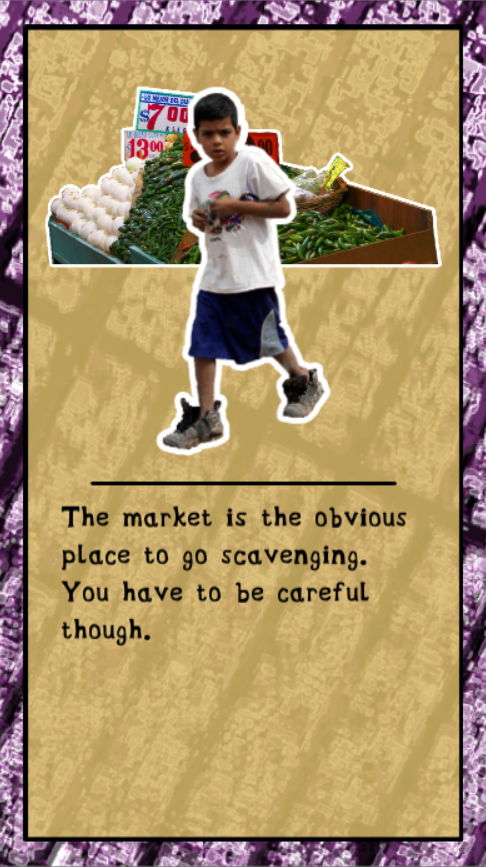
\includegraphics[width=0.5\textwidth]{GameScreen1.png}
    \caption{Story screen from the \textit{Rat Kid Dog Fight} prototype}
    \label{fig:GameScreen}
\end{figure}

%why did we choose which features?



\commenting{Choosing a vertical display for the phone for accessibility and to signal the briefness of the play session. insert this somewhere}


\subsection{Covering Prototype Limitations}
\label{limitations}
While we were creating a limited and deterministic prototype, we made several considerations, to hide the procedural and deterministic nature of the prototype. These include the map system, the ability to catch and breed, which all speak to a bigger game than the prototype is. The reason for doing this was to create an illusion of a longer game, and a potentially longer relationship with the dog. We feared that if the player knew the scale of the prototype or the already determined outcomes, they would not allow themselves to become emotionally attached to the dog. \\

To create this illusion the UI is not build for simply supporting the features of the prototype, but also to support the affordances a longer and less procedural game could include. The option to 'Breed' the dogs is a feature that is not actually included in the prototype, but since the player is forced to only catch dogs of one specific gender, they will never discover this.\\

\subsection{Lack of Player Agency in Fights}
As mentioned in \ref{Agency} we have implemented impotent options in the dog fights, which aims to create the illusion of agency. These options mimic the \textit{Pokémon} games, as seen in figure \ref{fig:PokeBattle} and \ref{fig:DogFightBattle}. 

\begin{figure}[h!] 
	\centering
    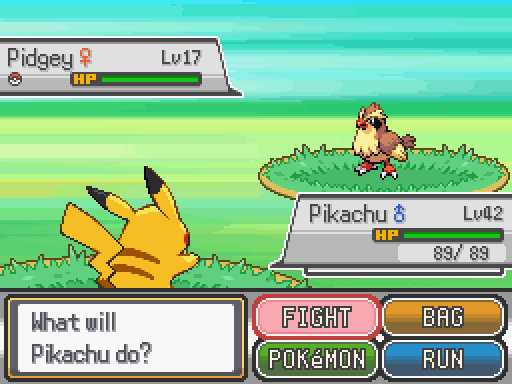
\includegraphics[width=0.5\textwidth]{PokemonBattle.png}
    \caption{A \textit{Pokémon} battle}
    \label{fig:PokeBattle}
\end{figure}

\begin{figure}[h!]
	\centering
    \includegraphics[width=0.5\textwidth]{battle.png}
    \caption{A \textit{Rat Kid Dog Fight!} battle}
    \label{fig:DogFightBattle}
\end{figure}

All these battle options does not have any effect on the actual battle. The \textit{Fight} option let the player select between \textit{Throat Bite}, \textit{Tackle}, \textit{Scratch} and \textit{Lock Bite}. While \textit{Scratch} and \textit{Tackle} are typical generic \textit{Pokémon} moves, the other two also resemble names of moves \textit{Pokémon}, with a dog fight appropiate connotation, which also makes them appear more visceral and brutal. When chosen, all of these fight-options simply give the text feedback of your character shouting something appropiate, like "Go for the throat, DOGNAME!" for selecting \textit{Throat Bite}, which also is a mediation of the television series \textit{Pokémon: The Series} (1997), where the main character, \textit{Ash}, could shout "Pikachu, use Thunderbolt!". This reference further creates the expectance of an actual effect on gameplay, since those familiar with the show, would know that there is always a direct link between what the Pokémon trainer shouts and what the Pokémon does and would expect the same causality here.
The option \textit{item} simply states that the player has no items to use and then progresses the battle. Likewise, the option \textit{Dog} states that the player "... cannot change dogs during this fight.". Similar to the (lacking) features mentioned in \ref{limitations}, this gives the player an idea of a bigger game, where they might unlock these options later on.\\

The goal with creating this illusion of player agency is to create a feeling of helplessness and hopefully the realization of no agency will put them in the place of the kid. 
\commenting{ref to 'Papers, Please'}
We want to battles to be realistically random\commenting{different word} and brutal, while still giving the player the illusion of being able to change the inevitable, creating the same superstition as mentioned in \ref{Agency}.\\

\subsection{Battle System}
Even though the player has limited agency in the fight system, we still simulate the fights with a very game-like system.\\

\begin{figure}[h!]
	\centering
    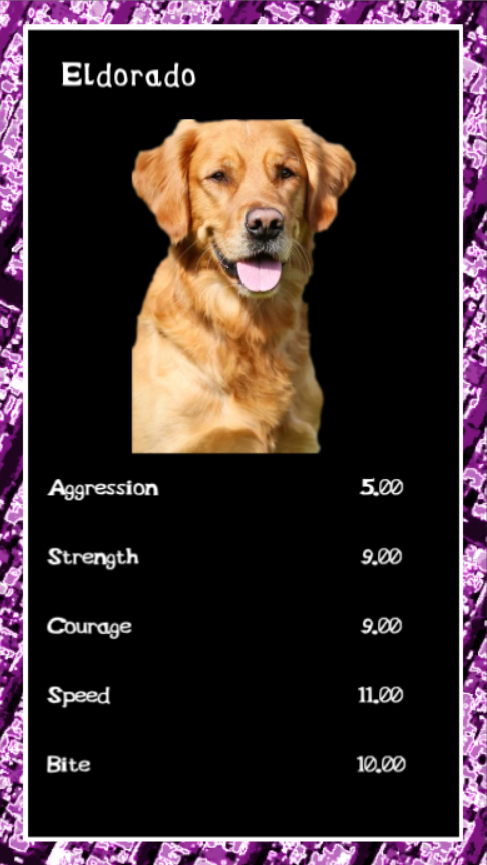
\includegraphics[width=0.5\textwidth]{DogStats.png}
    \caption{A dog stat screen from the \textit{Rat Kid Dog Fight!} prototype}
    \label{fig:DogStatScreen}
\end{figure}


The dogs has the following 5 stats: \textit{Aggression}, \textit{Strength}, \textit{Courage}, \textit{Speed} and \textit{Bite}.\\

The battle system works in the following way



\begin{center}
\scriptsize 
	\begin{tabular}{|l|p{5cm}|p{3cm}|p{3cm}|} 
		\hline
		\textbf{Game Round} & \textbf{Description} & \textbf{Example Outcome} &\textbf{ Feedback }\\ [0.5ex] 
		\hline\hline
		Aggression Roll & Each dog has a an aggression score. The one with the highest aggression will decrease the other dogs strength speed and bite depending on the others courage rating & Dog1s 10 AGGRESSION goes against Dog2s 6 courage and decreases Dog2s STRENGTH, SPEED and BITE by 40\% & "Dog2 is intimidated by the vicious barking from Dog1" \\  
		\hline\hline
		\textit{\textbf{Main loop}} \\
		\hline
		Speed Roll	& The dog with the highest roll, determined by speed bites first. &	Dog1 bites first & "Dog1 snaps after Dog2s neck. \\
		\hline
		Bite roll & The biting dogs rolls BITE against STRENGTH to penetrate to kill or injur the other dog. Max roll will always penetrate, Penetrating rolls has a chance to kill or injur the other dog. Non-penetrating rolls will still have the dog bite onto and get stuck in the other dog. Low rolls will not even get stuck & Dog1 bites onto Dog2. Locking it's jaws around it. The strength of Dog2 decreases.	& "Dog1 Bites Dog2. Its jaws locking onto the skin of Dog2s stomach." \\
		\hline
		Other dogs bite Roll & Similar to above, but with penalty if the other dog has biten onto it. & & "Dog2 bites Dog1. Its jaws locking onto the skin of Dog1s neck." \\
		\hline
	\end{tabular}
\end{center}

\commenting{correct bite roll explanation}

If a dog has its bite locked around the other one ...

If the jaws of both dogs are locked onto eachother
which simulate real dog fighting.

The main loop continues untill one of the dogs has 0 \textit{Strength}, after which the dog dies

\subsection{Actions Between Fights}
By only allowing one choice per game week, we implicitly associate a cost with the action, and an investment in your dog. In \cite{game:pokemon}



\section{Testing}
\subsection{Method}
To answer our hypotheses we have designed a qualitative play experience test. The procedure of the test includes first a playthrough of the game and then a semi-structured interview. The in-game choices made by the player in the playthrough is recorded as is their body language, statements or other sounds produced while playing.

The test subjects will be asked to participate in one playthrough of the game followed by a semi-structured interview to gather data on that specific play experience. Due to the mature content of the game the targeted test subjects are age 18 or above. To look for trends across genders we aim for gender equality in our sample. Furthermore while recruiting test subjects we look for subjects who has outspoken opinions about dogs, animal rights and/or human rights. The only quantitative data collected is the in-game choices of the game and these are of binary quality at best. 

In-game choices:
In the game you as player has to take several choices regarding the fate of your avatar. \commenting{Avatar or character?? it seems like it depends on the eyes that sees.. INVESTIGATE}

\subsection{Sessions}
Two testing sessions were conducted on the IT University of Copenhagen. The first on the 30th October 2017, the second on the 23rd November 2017. The test procedure followed the same guidelines for both of the tests however a few of the questions were rephrased and the implementation of the game underwent several changes. The changes included correction of spelling in the narrative, more graphical elements depicting the situation of the state of the game and better feedback in the dog fights in the game. These changes will have biased the test results and should be kept in mind when analysing the data.

A playthrough of the game took 10-15 min. depending on the speed of the participant - reading, taking decisions - and the random outcomes of the fights in the game. While playing the participants in-game choices was recorded. Some participants came to an end of the game after the second fight of the game others after the third.
The interview was conducted following af semi-structured questionnaire consisting of 17 predefined questions, participant demographics questions and a small observational sheet to record the actions taken by the participant in the game. Furthermore observations of the participants body language, statements and other kinds of sounds while playing the game was recorded.

\subsection{Results}
In total nine subjects, four male and five female, successfully participated in the test. The youngest being 24 and the oldest 31, average being 27,2 years old. Six of the participants are higher education students, two are film directors and the last participant is educated but unemployed. It is safe to conclude that the participants on average possesses intellectual judgement.

The most important choice of the game is where the player is asked to choose their destiny. Whether they will participate in dog fighting or offer sexual favours to earn money. Six participants chose dog fighting, three chose sexual favours. All but one of the participants made the choice relatively quickly between three to nine seconds. The one exemption spend a minute before choosing dog fighting.

\subsection{Discussion}
In the following paragraph test subjects will be referred to by number 1-9. 

IS DOG FIGHTING THE BETTER ALTERNATIVE?
One of the things we were curious about is whether dog fighting is perceived as a better alternative to prostitution. It is no secret that in our - the designers - mind dog fighting is a better alternative. Our test data indicate that the majority of the participants felt the same way but we cannot ignore the data that resists this notion. A trend in the data reveals that the visual appearance of the man you are to prostitute yourself to has had an impact on the choice. We might also have to question whether the choice is affected by the player's cultural background.

One participant(2) spend a minute making the decision. She was clearly emotionally affected by the game and the choice made her feel uncomfortable. Interestingly she was part of the first test session. In the implementation of the game used for the first session the man to which you can offer sexual favours is not depicted. In the second implementation of the game he is depicted as being very repulsive.  \commenting{Insert picture of man} The fact that he is not depicted in the first test session may have made the choice less unambiguous. This thought is supported by two other participants(7, 9) statements to the question "Why did you pick dog fighting over sexual favours?". They state that the man's uglyness played a role in their decision to pick dog fighting. A fourth participant(8) states that he felt the game wanted him to choose dog fighting over sexual favours. Whether the depiction of the man has had an impact on this can only be speculated but it seems like the new implementation of the game pushes the player more towards picking dog fighting over sexual favours.

Two(1, 6) of the three participants who chose sexual favours over dog fighting stated that they chose sexual favours out of curiosity. Observations of the participants, a male and a female, indicate that they were taking the seriousness of the game lightly and were having fun with it. They seemed to have a satirical distance to the game. The male participant(1) states that he chose the sexual favours because it was more extreme. The female(2) states that her choice may have been biased because she was sitting at a test. Their data indicate that they felt that dog fighting was the moral choice but that they chose sexual favours just to see what would happen in the game. Interestingly the last participant(4) chose sexual favours because she felt that it was the moral choice. Born and raised in Hong-Kong her cultural background is different from the rest of the participants (native Danes). Her reasoning being that no one dies in the sexual favours scenario. She is aware of, and believes that her opinion and choice is different from the other test participants. However she herself states that it is because of her cultural background.

CHARACTER / AVATAR AND DOG
A central question regarding the game design is how emotionally invested the players are in the game. Our goal was to create a play experience that had en emotional impact on the player that goes beyond pure entertainment. We believed that this could be achieved by first creating a gloomy narrative set in a - close to - real environment and by creating affordances that makes the player experience the story as being the protagonist rather than observing.  The participants identification with the depicted protagonist of the game and the participants perceived roles in the game indicates that the participants played the game in different ways. We cannot quantify the participants emotional investment but there are trends in the data that indicate how the players felt while playing the game. The data indicates that the players have different perceptions of the protagonist as an avatar. To some he is a rounded character whos fate the players decide, to others he is a projection of player's self in his reality. To avoid a confusion of the character versus the avatar we will refer to the protagonist as the 'protagonist' in the following paragraph.

The second decision the participants had to make in the game was to give the protagonist a name. Six participants(1, 2, 3, 4, 5, 7) chose to give the protagonist a what we define as a serious name. The serious names are names that resemble the participants real name or is a known nickname of theirs while the non-serious names are not. We speculate that the participants chose a serious name because they want to identify with the protagonist rather than distance themselves from him. While picking a non-serious name is a way to create a humorous distance between yourself and the protagonist in the game. This speculation is partly supported by the data. One of the participants(6) who chose a non-serious name was experiencing the whole game as a satire, she clearly had a humorous distance to the entire play experience. Another participant(9) who chose a non-serious name states that he did not identify with the protagonist and that it was a conscious decision to give the protagonist a non-serious name. However data from three of the participants(1, 4, 7) who chose a serious name indicates that they did not identify with the protagonist. Hence the name to protagonist relationship hypothesis does not seem to apply. Instead choosing a serious name may be an expression of how willing you are to invest emotions in the game.

Interestingly the serious name pattern changes when the participants are asked to give their dog a name. Now only two participants(2, 7) chose to give their dog a serious name. This shift might indicate either that the game has made the participants perceive their role in the game differently or that the participants are trying consciously to distance themself from the either the game or the dog in the game. Participant 5 and 9 states that they chose a funny or distancing name to avoid getting too close to the dog. The data of participant 4 indicate the same trend but is less clear cut. Participants 1, 3 and 8's data indicate that they did not yet feel attached to the dog the moment they had to give it a name. Participant 6 was as explained earlier having a satirical distance to the entire game experience.
Interestingly only two participants(6, 8) chose to leash the dog however both of them expressed that they thought it was the correct option, implying that they were afraid of the consequences if they did not leash it. Participant 1, 2, 3, 7 and 9 express that they believe their relationship with the dog would be improved by not leashing it. Participant 4 and 5 both express that leashing it would have made the dog easier to control, but chose to not leash it. The findings indicate that the name can be perceived as an indication of emotional engagement in the game. Moreover it seems that our implementation did a sub par job at creating the necessary emotional bonding to the dog prior to the naming of it.


CAN WE CREATE UNETHICAL AFFORDANCES, NAMELY DOG FIGHTING, IN A GAME WITHOUT MAKING IT AN UNETHICAL GAME?

To the question "Do you think it was an unethical game?", six participants(1, 2, 3, 4, 7, 9) answered no, two(5, 8) answered yes and one(6) answered that it did not matter as the game is satire. Participant 5 elaborates that he believes the Mexicans will oppose the game, but that in a sense the game is not more unethical than other games. He believes that human fights is more unethical, implying that the while unethical the game can exist under the socially accepted unethical threshold of games. Participant 8 elaborates that the humor in the game makes it very unethical, but that its existence is still justified. Participants 1, 2, 3, 4 & 7 elaborates that the game makes you are aware and puts you in the horrible situation of the game, implying that your actions are justified by the situation you are in. Participant 4 and 7's only real complaint was that they wanted a disclaimer for the blood on the dogs.
When asked if the game was moralising seven participants(1, 2, 3, 5, 6, 8, 9) answered no, one(4) answered yes and the last one(7) was not sure. Participants 1, 2, 3 and 5 elaborates that the game itself does not tell you what is right or wrong. Participant 4 states that the game is trying to hint something. She is not defining what the game is hinting but says the game is made to make you feel bad by dismembering and putting blood on cute dogs. Participant 7 also cannot define what the moral of the game is but that it is hard that the game forces her to downprioritise her dog. 


WILL THE PLAYER BE ABLE TO FEEL EMPATHY FOR THE DOGS, WHILE BEING RELIANT ON THEM FIGHTING?

The participants choice of dog described in their responses to the question "Why did you pick the dog you picked?" are coded as being either a choice based on feelings or rationale. Six participants(2, 3, 4, 5, 6, 7, 9) made a rational decision on their choice of dog. They base their decision on which dog they felt was best capable of fighting. In contrary participant 1 and 8 based their choice of dog on feelings. Participant 1 chose the husky because he thought it was cool but speculate that the boxer might have been more capable of fighting. Participant 8 did not choose the boxer because he was too emotionally attached to it and he wouldn't want to see it suffer. His response raises the question whether the other participants seemingly rationale choices are made on the basis of choosing the dog that would suffer the least. If that is the case then the participants choices are based on feelings in the sense that they choose the dog that will have the least emotional impact on them.



\begin{table}[h]
\centering
\begin{tabular}{l l l}
\hline
\textbf{Destiny} & Sexual favours & Dog fight\\
\hline
Male & 1 & 2 \\
Female & 4 & 2 \\
\hline
\end{tabular}
\caption{Table caption}
\end{table}

A cross reference to table \ref{tab:one}
\begin{table}
\begin{tabular}{|c|c|c|}
\hline 
 This & is & a table \tabularnewline
\hline 
\end{tabular}
\caption{\label{tab:one}The caption of table one}
\end{table}



TO-DO:...
Take the previous written stuff and see if it fits as answers to the three hypotheses. Find more trends in the data. Structure the whole testing paragraph in a better way. At least make subsection titles better. Get more into agency versus avatar versus character and use proper references.
ie. 

Wardrip-Fruin, Noah et al. (2009): "Agency Reconsidered.? Breaking New Ground: Innovation in Games, Play, Practice and Theory. Proceedings of DiGRA 2009, URL: http://www.digra.org/digital-library/publications/agency-reconsidered/

Linderoth, Jonas. (2005): Animated game pieces. Avatars as roles, tools and props. In Aesthetics of Play Conference Proceedings, URL: http://www.aestheticsofplay.org/linderoth.php

Klevjer, Rune (2012): "Enter the Avatar: The Phenomenology of Prosthetic Telepresence in Computer Game?. In The Philosophy of Computer Games (pp. 17-38). Springer Netherlands.






\section{Future Game Mechanics}
\commenting{maybe find another title}
\label{Future}
In this section we will discuss under which conditions the prototype would be best evolved into an actual game.

\subsection{Game Mechanics}
From the test results in section \ref{testResults}

Setting seemed to work very well. \commenting{ethics book reference} Could be shortened or shown more cinematically.\

the selection of sex or dog fight could be done by the character, as in many games (ref gta), as to not make a street kid simulator.\

As mentioned in \ref{testResults} none of our testers understood, that there was no agency in the battles, while they did comment on a lack of understanding of how the selectable options worked. It should therefore be possible to make combat actually have agency, without the game becoming too unethical. Still, we believe the gameplay would be better served without any agency in the battle, where the player knows that there is not any agency. Instead the player could have the possibility of having the player character shout different commands to the dog in the battles. This could be similar to the shouts from the actions we have currently, as mentioned in \ref{Design}. This would more legitimately position the player in the same position as the kid, hoping that the shouts might change something, instead of expecting it.\

Instead of combat agency the gameplay should focus on the places where the player actually is able to make an impact; training, breeding, catching dogs, economy management and random events. Here the player should be able to strategize and plan, so the important part would be which dogs they pit against which, catching or breeding good fighting dogs, and chosing when the stakes are high enough to throw your prime bitch into the ring. This should allow for plenty of design space for strategy and actual gameplay, while still keeping the realism and brutality of the fights. \

Less humour and pokémon references could make it a more ethical game. \commenting{elaborate}\

\subsection{Audience and Platform}

As mentioned in \ref{testResults}, one of our testers even suggested collaborating with NGO's, to create awareness around the conditions of street kids and illegal dog fighting. \

For the platform we believe both art exibitions, schools and retail release could all be possible. Interestingly, we believe that the latter would need more attention to the ethical considerations, possibly even necessitating the downgrade of some of the systems to a less game-like structure. On the other hand developing the game as an art project, meant to be shown at a museum or art exibition, would just by the context establish the game as a piece of art, and allow, possibly even expect, more extreme forms of expression, in regards to humour and affordances.
A game where the intended purpose is either educational or artistic, would also be easier to find funding for. 
Hence, we find that an initial release for either schools or museums, with the possibility of a later retail release on Steam\footnote{\url{http://store.steampowered.com/}} would be ideal.\

One problem with collaborating with schools or NGO's, is that the players might find the game more moralizing, even if would not in another context, simply because of these associations. No matter which platform is chosen, it is important that the features reflect the audience and agenda, especially since people are very influenced by this subject matter, as we witnessed in testing.\



\section{Conclusion}





%% The Appendices part is started with the command \appendix;
%% appendix sections are then done as normal sections
\appendix

\section{Appendix}
\label{appendix}

%% References
%%
%% Following citation commands can be used in the body text:
%% Usage of \cite is as follows:
%%   \cite{key}          ==>>  [#]
%%   \cite[chap. 2]{key} ==>>  [#, chap. 2]
%%   \citet{key}         ==>>  Author [#]

%% References with bibTeX database:

\bibliographystyle{model1-num-names}
\bibliography{sample.bib}

%% Authors are advised to submit their bibtex database files. They are
%% requested to list a bibtex style file in the manuscript if they do
%% not want to use model1-num-names.bst.

%% References without bibTeX database:

% \begin{thebibliography}{00}

%% \bibitem must have the following form:
%%   \bibitem{key}...
%%

% \bibitem{}

% \end{thebibliography}


\end{document}

%%
%% End of file `elsarticle-template-1-num.tex'.